\documentclass[dvipdfmx]{beamer}
\usepackage{tutorial}
\title{計算機実験 --- 最適化問題}

\begin{document}

\lstset{language={C},basicstyle=\ttfamily\scriptsize,showspaces=false,rulecolor=\color[cmyk]{0, 0.29,0.84,0}}

\begin{frame}
  \titlepage
  \tableofcontents
\end{frame}

% -*- coding: utf-8 -*-

\section{最適化問題}

\begin{frame}[t,fragile]{最適化問題}
  \begin{itemize}
    %\setlength{\itemsep}{1em}
  \item 目的関数(コスト関数)$f(x)$の最小値(あるいは最大値)とその場所を求めたい
  \item どういう問題を解くのに使えるか?
    \begin{itemize}
    \item 変分原理が成り立つ問題: 最小作用の原理、最小エネルギーの原理$\cdots$
    \item 目的関数が定義できる問題: 最小二乗法(線形回帰、非線形回帰)、(連立)方程式、常/偏微分方程式、機械学習$\cdots$
    \end{itemize}
  \item ほぼ全ての問題は、目的関数をうまく定義することで最適化問題に書き換えることができる
    \begin{itemize}
    \item (一般に)最適化問題として解くのは最終手段
    \item それぞれの問題に特化したより良い方法があるときはそちらを使う
    \end{itemize}
  \end{itemize}
\end{frame}

\begin{frame}[t,fragile]{様々な最適化手法}
  \begin{itemize}
    %\setlength{\itemsep}{1em}
  \item 最適化問題の種類
    \begin{itemize}
    \item 連続最適化問題 $\Leftarrow$ 目的関数が凸ではない場合、難しい
    \item 離散最適化(組み合せ最適化)問題 $\Leftarrow$ さらに難しい
    \end{itemize}
  \item 真の(大局的な)最小値(最大値)を求めるのは難しい
  \item 一般的には極値を求めることしかできない
  \item 多次元では極小を囲い込むことができない
  \item 導関数を使う方法: ニュートン法、準ニュートン法、最急降下法、勾配降下法、共役勾配法$\cdots$
  \item 使わない方法: 囲い込み法、Nelder-Meadの滑降シンプレックス法、シミュレーテッドアニーリング、量子アニーリング$\cdots$
  \item 目的関数・導関数の評価回数と収束までの反復回数のトレードオフ
  \end{itemize}
\end{frame}


\section{囲い込み法}

\begin{frame}[t,fragile]{囲い込み法(一次元の最適化)}
  \begin{itemize}
    \setlength{\itemsep}{1em}
  \item $f(a) > f(b) < f(c)$を満たす3点の組$a < b < c$の領域を狭めていく
  \item $[a,b]$、$[b,c]$の広い方(例えば後者)を$b$から見て、黄金比
    [$1:(1+\sqrt{5})/2 \approx 0.382:0.618$]に内分する点を$x$とする
    \begin{itemize}
    \item $f(b) > f(x)$の場合: $[b,c]$を新しい領域にとる
    \item $f(b) < f(x)$の場合: $[a,x]$を新しい領域にとる
    \end{itemize}
  \item もともとの$b$が$[a,c]$を$0.382:0.618$に内分する点だった場合、
    新しい領域の幅は、どちらの場合も0.618
  \item 最初の比率が黄金比からずれていたとしても、黄金比に収束
  \item 黄金分割法(golden section)とも呼ばれる
  \end{itemize}
\end{frame}

\begin{frame}[t,fragile]{最初の囲い込み}
  \begin{itemize}
    \setlength{\itemsep}{1em}
  \item 1点を選び、適当な$\Delta x$を取る
  \item 左右に$\Delta x$動かしてみて、関数値が小さくなる方へ動く
  \item どちらに進んでも関数値が大きくなる場合には、囲い込み完了
  \item 小さくなった場合、その方向へ再び増えるまで$\Delta x$を倍々に増やしながら進む
  \item 最後の3点で極小値を囲い込むことができる
  \item 囲い込み法のプログラムの例: \href{https://github.com/todo-group/computer-experiments/blob/master/exercise/optimization/golden_section.c}{golden\_section.c}
  \end{itemize}
\end{frame}

\begin{frame}[t,fragile]{極小値をとる$x$の精度}
  \begin{itemize}
    \setlength{\itemsep}{1em}
  \item 実数の有効桁数を16桁($\epsilon \approx 10^{-16}$)とする(倍精度)
  \item 真の極小($x_0$)のまわりでテイラー展開
    \[
    f(x) \approx f(x_0) + \frac{1}{2} f''(x_0) (x-x_0)^2
    \]
  \item $f''(x_0) / f(x_0)$が$O(1)$だとすると
    \[
    |x-x_0| \sim \sqrt{\epsilon} \sim 10^{-8}
    \]
    以下になると、第二項の第一項に対する比が$\epsilon$よりも小さくなる
  \item それ以上領域を狭めても、関数値は変化しない
  \end{itemize}
\end{frame}

\section{最急降下法と勾配降下法}

\begin{frame}[t,fragile]{最急降下法(steepest descent)}
  \begin{itemize}
    \setlength{\itemsep}{1em}
  \item 関数の微分の情報を使う
  \item 現在の点$\bf x$における勾配を計算
    \[
    -\nabla f|_i = -\frac{\partial f}{\partial x_i}
    \]
  \item 坂を下る方向にそって、一次元最適化
  \item 動いた先の勾配の方向でさらに最適化を繰り返す
  \item 関数値は単調減少 $\Rightarrow$ 極小値に収束
  \end{itemize}
\end{frame}

\begin{frame}[t,fragile]{勾配降下法(gradient descent)}
  \begin{itemize}
    \setlength{\itemsep}{1em}
  \item 勾配方向に一次元最適化を行うかわりに、あらかじめ決めた一定量($\epsilon$)だけ坂を下る
    \[
    x_{n+1} = x_n - \epsilon \, \nabla f
    \]
  \item あらかじめ最適な$\epsilon$を知るのは困難
  \item 機械学習の分野では、(なぜか) $\epsilon=0.1$が良いとされている
  \item この方法を「最急降下法」、一次元最適化を行う勾配法を「最適降下法(optimum descent)」と呼ぶ場合も
  % \item c.f.) 確率的勾配降下法(stochastic gradient descent)
  \end{itemize}
\end{frame}

\begin{frame}[t,fragile]{制約条件付きの場合}
  \begin{itemize}
    % \setlength{\itemsep}{1em}
  \item 目的関数: $f(x)$
  \item 制約条件:
    \begin{itemize}
    \item $g_i(x) = 0$ \ ($i=1,\cdots,m$) \ (等式制約条件)
    \item $h_j(x) \ge 0$ \ ($j=1,\cdots,n$) \ (不等式制約条件)
    \end{itemize}
  \item 等式制約条件の付いている場合: Lagrangeの未定乗数法
    \[
    L(x,\lambda_1,\cdots,\lambda_m)=f(x)+\sum_i \lambda_i g_i(x)
    \]
    を考え、$x,\lambda_1,\cdots,\lambda_m$に関する微分が零となる点を探す
  \item 不等式制約条件の付いている場合: 線形計画法, ペナルティ関数法
  \end{itemize}
\end{frame}

\begin{frame}[t,fragile]{細長い谷の場合}
  \vspace*{1em}
  \hspace*{1em}\resizebox{1\textwidth}{!}{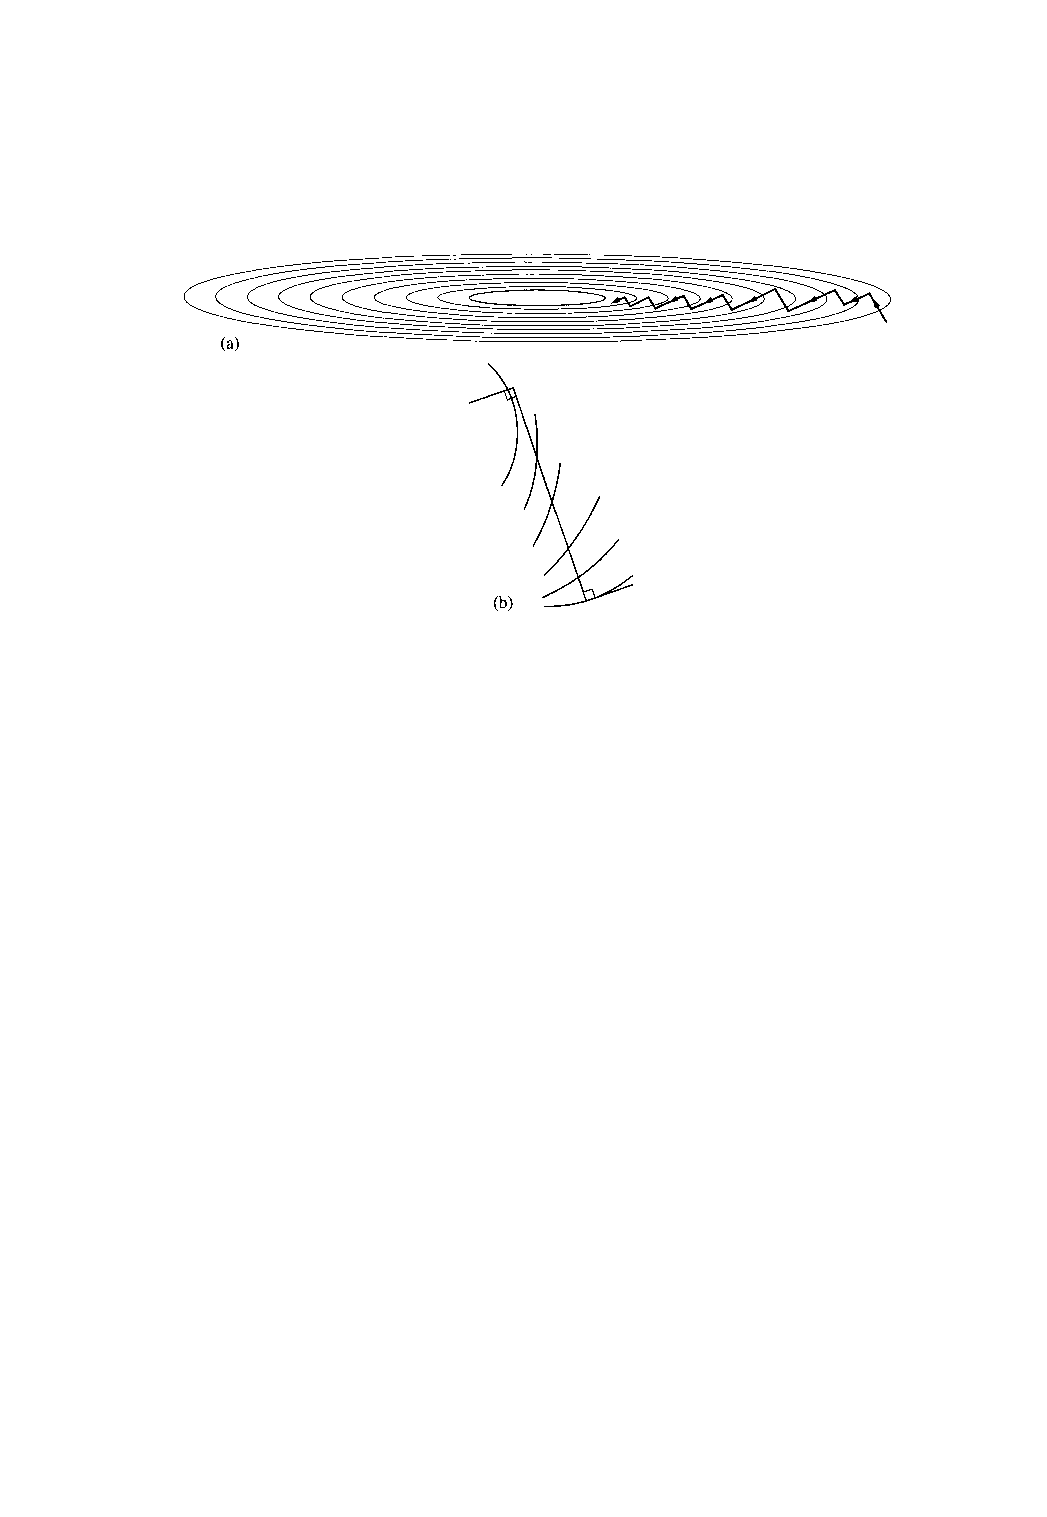
\includegraphics{image/steepest-descent.pdf}}

  \vspace*{-2em}
  \hspace*{20em}{\footnotesize(Press et al 1988)}
\end{frame}

% -*- coding: utf-8 -*-

\section{共役勾配法}

\begin{frame}[t,fragile]{共役勾配法(conjugate gradient)}
  \begin{itemize}
    \setlength{\itemsep}{1em}
  \item $d$次元空間の目的関数$f({\bf x})$がある点のまわりで
    \[
    f({\bf x}) \approx c - {\bf b}^T {\bf x} + \frac{1}{2} {\bf x}^T A {\bf x}
    \]
    と近似できるとする
  \item ${\bf x}$における勾配は、連立方程式$A{\bf x}={\bf b}$の「残差」の形で書ける
    \[
    -\nabla f = {\bf b} - A {\bf x}
    \]
  \item 新しい勾配方向ではなく、それまでとは「共役な方向」に進みたい
  \end{itemize}
\end{frame}

\begin{frame}[t,fragile]{「共役な方向」とは}
  \begin{itemize}
    \setlength{\itemsep}{1em}
  \item あるベクトル${\bf p}$にそった一次元の最適化が完了したとする
    \begin{itemize}
    \item その点における${\bf p}$方向の勾配は零。すなわち${\bf p}^T (\nabla f)=0$
    \item ${\bf p}$方向の勾配の値を変化させないようにしたい
  \end{itemize}
  \item 次に、${\bf q}$にそって、${\bf x}+\epsilon {\bf q}$と移動するとする。その時の勾配の変化は
    \[
      \delta(\nabla f) = A \times (\epsilon {\bf q}) \sim A {\bf q}
      \]
      これが${\bf p}$に垂直であるためには
    \[
      {\bf p}^T A {\bf q} = 0
      \]
    \item この関係が成り立つ時、${\bf p}$と${\bf q}$は「互いに共役」という
  \end{itemize}
\end{frame}

\begin{frame}[t,fragile]{共役勾配法(conjugate gradient)}
  \begin{itemize}
    \setlength{\itemsep}{1em}
  \item 初期条件: 位置 ${\bf x} = {\bf x}_0$
    \begin{align*}
      & \text{勾配:} \ {\bf p} = {\bf p}_0 = -\nabla f({\bf x}_0) = {\bf b} - A {\bf x}_0 \\
      & \text{残差:} \ {\bf r} = {\bf r}_0 = {\bf p}_0
    \end{align*}
  \item 最適化(第$n$ステップ)
    \begin{align*}
      \alpha_n &= \frac{{\bf r}_n^T {\bf p}_n}{{\bf p}_n^T A {\bf p}_n} \\
            {\bf x}_{n+1} &= {\bf x}_n + \alpha_n {\bf p}_n \\
            {\bf r}_{n+1} &= {\bf r}_n - \alpha_n A {\bf p}_n = {\bf b} - A {\bf x}_{n+1} \\
            \beta_n &= - \frac{{\bf p}_{n}^T A {\bf r}_{n+1}}{{\bf p}_n^T A {\bf p}_n} \\
                 {\bf p}_{n+1} &= {\bf r}_{n+1} + \beta_n {\bf p}_n
    \end{align*}
  \end{itemize}
\end{frame}

\begin{frame}[t,fragile]{共役勾配法 - 直線上の最適化}
  \begin{itemize}
    \setlength{\itemsep}{1em}
  \item 直線${\bf x} = {\bf x}_n + \alpha {\bf p}_n$上での最適化
  \item 点${\bf x}$で$f({\bf x})$が最小値をとるためには、${\bf x}$における勾配と直線の方向ベクトル${\bf p_n}$が垂直にならなければならない
    \begin{align*}
      -[\nabla f({\bf x})]^T {\bf p}_n &= ({\bf b} - A {\bf x})^T {\bf p}_n
      % = {\bf r}^T {\bf p}_n
      = ({\bf b} - A ({\bf x}_n+\alpha {\bf p}_n))^T {\bf p}_n \\ &= ({\bf r}_n - \alpha A {\bf p}_n)^T {\bf p}_n = 0
    \end{align*}
    %(${\bf r}_n \equiv {\bf b} - A{\bf x}_ n$)
  \item 最適解: $\displaystyle \alpha_n = \frac{{\bf r}_n^T {\bf p}_n}{{\bf p}_n^T A {\bf p}_n}$
  \end{itemize}
\end{frame}

\begin{frame}[t,fragile]{共役勾配法 - 共役な方向の決め方}
  \begin{itemize}
    \setlength{\itemsep}{1em}
  \item 新たな最適化方向: ${\bf p} = {\bf r}_{n+1} + \beta {\bf p}_n$
  \item $\beta=0$とすると最急降下法と等価
  \item 共役勾配法では、${\bf p}$と${\bf p}_{n}$が共役となるように$\beta {\bf p}_n$だけ補正を加える
    \begin{align*}
      {\bf p}_n^T A {\bf p} = {\bf p}_n^T A ({\bf r}_{n+1} + \beta {\bf p}_n) = 0
    \end{align*}
  \item $\beta$について解くと
    \begin{align*}
      \beta_n &= - \frac{{\bf p}_{n}^T A {\bf r}_{n+1}}{{\bf p}_n^T A {\bf p}_n}
    \end{align*}
  \end{itemize}
\end{frame}

\begin{frame}[t,fragile]{共役勾配法 - 共役性と直交性}
  \begin{itemize}
    \setlength{\itemsep}{1em}
  \item 共役性: $\{{\bf p}_i\}$は自動的に互いに共役となる
    \begin{align*}
      {\bf p}_i^T A {\bf p}_j &= 0 \qquad \text{($i < j \le n$)}
    \end{align*}
  \item ${\bf x}_n$を通り${\bf p}_0 \cdots {\bf p}_n$に並行な「平面」上で$f({\bf x}_{n+1})$は最小
    \begin{align*}
      {\bf p}_i^T {\bf r}_{n+1} &= 0 \qquad \text{($i \le n$)}
    \end{align*}
  \item 直交性: $\{{\bf r}_i\}$は自動的に互いに直交する
    \begin{align*}
      {\bf r}_i^T {\bf r}_j &= 0 \qquad \text{($i < j \le n+1$)}
    \end{align*}
  \item $N$回反復すると残差は零 (実際は数値誤差により直交性がくずれる)
  \end{itemize}
\end{frame}

\begin{frame}[t,fragile]{最適化問題として連立一次方程式の解を求める}
  \begin{itemize}
    %\setlength{\itemsep}{1em}
  \item 行列$A$を正定値対称行列とする
  \item 連立方程式$A{\bf x}={\bf b}$の解を$\hat{\bf x}$とすると、目的関数
    \begin{align*}
      f({\bf x}) = \frac{1}{2} (\hat{\bf x} - {\bf x})^T A (\hat{\bf x} - {\bf x})
    \end{align*}
    は${\bf x} = \hat{\bf x}$の時、最小値0をとる
  \item ${\bf x}$における目的関数の勾配は、連立方程式の「残差」の形で書ける
    \begin{align*}
      -\nabla f = A (\hat{\bf x} - {\bf x}) = {\bf b} - A {\bf x} \equiv {\bf r}
    \end{align*}
  \item $f({\bf x})$の値を計算するには真の解$\hat{\bf x}$が必要だが、$f({\bf x})$の値そのものではなく勾配のみがあれば良い
  \item 行列ベクトル積だけで計算できるので、$A$が疎行列の時、特に有効 ⇒ 共役勾配法を利用
  \end{itemize}
\end{frame}

\begin{frame}[t,fragile]{共役勾配法による一般の関数の最適化}
  \begin{itemize}
    \setlength{\itemsep}{1em}
  \item $f({\bf x})$は厳密な二次形式ではない
  \item 係数行列$A$も分からない
  \item $\alpha_n$は一次元最適化を使って反復法で求める
  \item $\beta_n$は、$A$を知らなくても計算可能
    \begin{align*}
      \beta_n &= \frac{{\bf r}_{n+1}^T {\bf r}_{n+1}}{{\bf r}_n^T {\bf r}_n}
    \end{align*}
  \end{itemize}
\end{frame}


% -*- coding: utf-8 -*-

\section{Nelder-Meadの滑降シンプレックス法}

\begin{frame}[t,fragile]{Nelder-Meadの滑降シンプレックス法}
  \begin{itemize}
    %\setlength{\itemsep}{1em}
  \item 関数値のみ。導関数の情報を必要としない
  \item プログラミングが簡単
  \item 収束は遅いが、安定に極小値が求まる
  \item $d+1$個の頂点からなる$d$次元の超多面体(シンプレックス)を変形しながら、極小値を探す
    \begin{itemize}
    \item 2次元: 三角形
    \item 3次元: 四面体
    \end{itemize}
  \item 別名「アメーバ法」
  \end{itemize}
\end{frame}

\begin{frame}[t,fragile]{Nelder-Meadの滑降シンプレックス法}
  \begin{itemize}
    %\setlength{\itemsep}{1em}
  \item $d+1$個の点$x_0,x_1,\cdots,x_d$は$f(x_0) \le f(x_1) \le \cdots \le f(x_d)$の順に並べられているとする
  \item 最大値を取る点$x_d$を除く$d$点の重心を$x_g$とする
  \item Nelder-Mead法では以下のステップを繰り返す
    \begin{itemize}
    \item $x_d$を$x_g$に関する対称な点$x_r$に移動(反射)
      \[
      x_r = x_g + (x_g - x_d)
      \]
    \item $f(x_r)$が$f(x_0)$よりも小さい場合、さらに先に進む(拡大)
      \[
      x_e = x_g + 2(x_r - x_g)
      \]
    \item $f(x_r)$が$f(x_{d-1})$よりもまだ大きい場合には、$x_d$を$x_g$に近づける(縮小)
      \[
      x_c = x_g + (x_d-x_g)/2
      \]
    \item $f(x_c)$が$f(x_d)$よりまだ大きい場合には、$x_0$以外の点を$x_0$に一様に近づける(収縮)
      \[
      x_i \leftarrow x_0 + (x_i-x_0)/2 \qquad (i=1 \cdots d)
      \]
    \end{itemize}
  \end{itemize}
\end{frame}

% -*- coding: utf-8 -*-

\begin{frame}[t,fragile]{Nelder-Meadの滑降シンプレックス法}
  \vspace*{-2em}
  \hspace*{1em}\resizebox{!}{1.0\textheight}{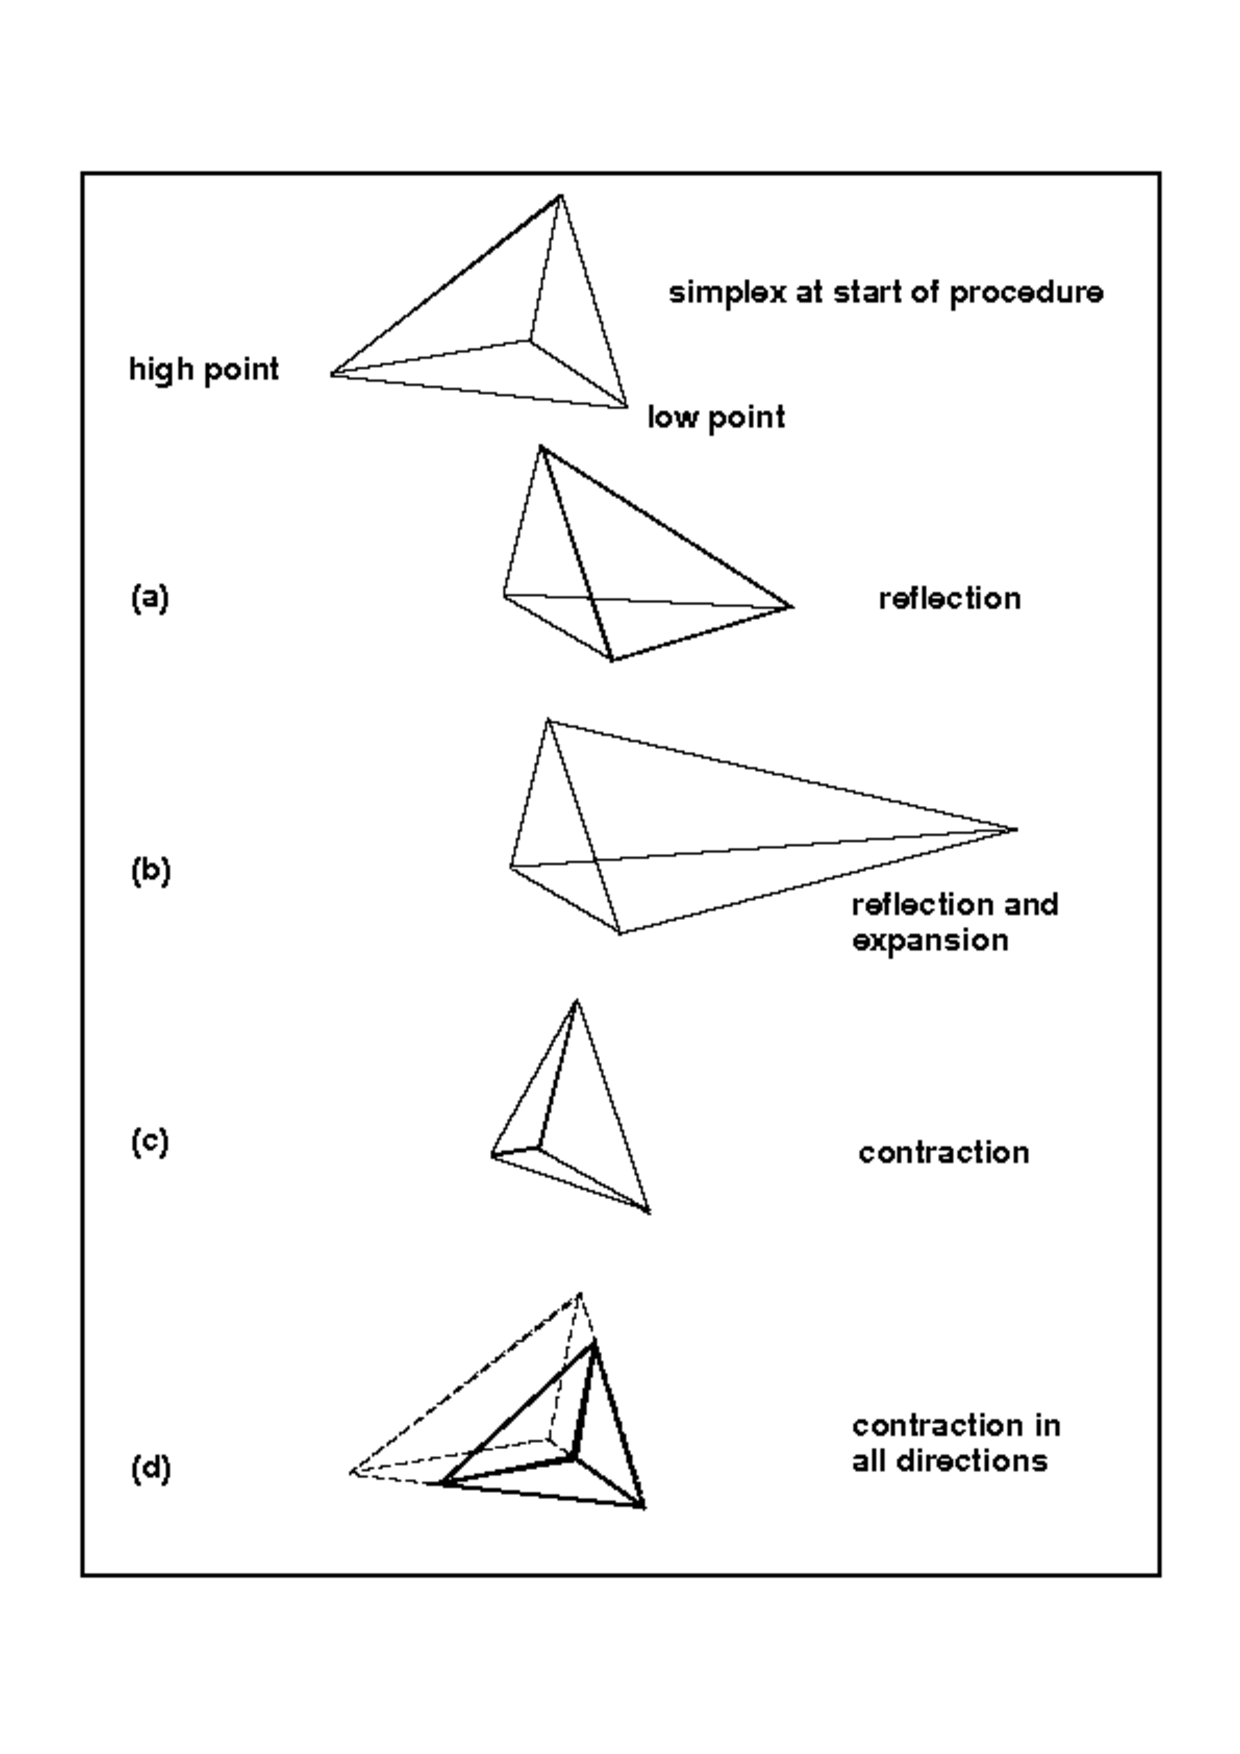
\includegraphics{image/neldermead.pdf}}

  \vspace*{-4em}
  \hspace*{18em}{\tiny\url{http://www.kniaz.net/software/RosNM.aspx}}
\end{frame}


\section{シミュレーテッド・アニーリング}

\begin{frame}[t,fragile]{確率過程を用いた最適化}
  \begin{itemize}
    \setlength{\itemsep}{1em}
  \item 最急降下法 (steepest decent) {\footnotesize \href{https://github.com/todo-group/computer-experiments/blob/master/exercise/optimization/mc_steepest_descent_1d.c}{example-2-L4/mc\_steepest\_descent\_1d.c}}
    \begin{itemize}
    \item 初期状態をランダムに定める
    \item 配位を少しだけ変化させる
    \item エネルギー(コスト関数)が小さくなるなら採択、大きくなるなら棄却
    \item 状態が変化しなくなるまでくり返す %$\Rightarrow$ 絶対零度でのMetropolis法
    \item 問題点 : エネルギー極小状態にすぐに捕まってしまう
    \end{itemize}
  \item 徐冷法 (simulated annealing) {\footnotesize \href{https://github.com/todo-group/computer-experiments/blob/master/exercise/optimization/simulated_annealing_1d.c}{example-2-L4/simulated\_annealing\_1d.c}}
    \begin{itemize}
    \item いきなり温度を零にするのではなく少しずつ下げていく
    \item どれくらいゆっくり下げれば良いか? $
      T(t) \ge cN / \log(t+2)
      $
    \item 実際には適当なスケジューリングで温度を下げ、何回か繰り返して最も良い結果を採択
    \end{itemize}
  \end{itemize}
\end{frame}

\begin{frame}[t,fragile]{最急降下法とシミュレーテッド・アニーリング}
  \noindent\resizebox{0.45\textwidth}{!}{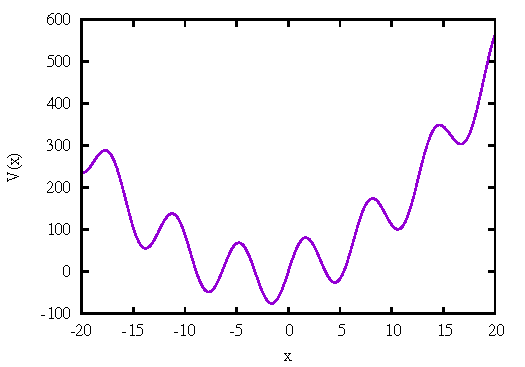
\includegraphics{image/potential.pdf}}

  \noindent\hspace*{.5em}\resizebox{0.43\textwidth}{!}{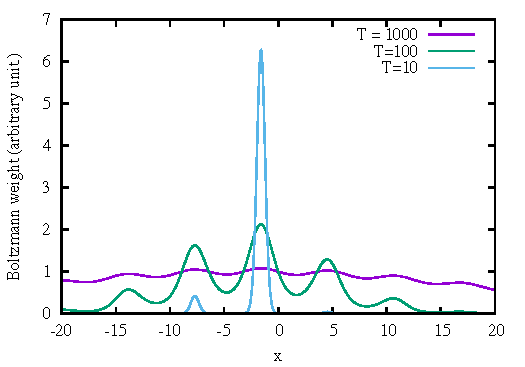
\includegraphics{image/boltzmann.pdf}}

  \vspace*{-17em}\hspace*{12.5em}\resizebox{0.6\textwidth}{!}{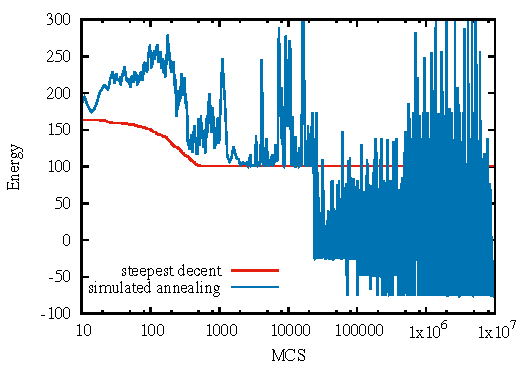
\includegraphics{image/energy.pdf}}

  \hspace*{17em}$T(t) = 100 - \frac{99}{10^7} t$
\end{frame}

\begin{frame}[t,fragile]{離散最適化問題への応用}
  \begin{itemize}
    \setlength{\itemsep}{1em}
  \item 微分を必要としないので、離散最適化問題にも適用可
    \begin{itemize}
    \item 例: 巡回セールスマン問題、数独、ナップザック問題
    \end{itemize}
  \item いかに状態とエネルギーを定義するかが重要
    \begin{itemize}
    \item 例: $n \times n$魔法陣 (行・列・ななめの和$M = n(n^2+1)/2$)
    \item 「状態」C: $1\sim n^2$の自然数をある順序でます目に並べたもの
    \item 「エネルギー」
      \[
      E(C) = \sum_{\rm row} (S_r-M)^2 + \sum_{\rm col} (S_c-M)^2 + \sum_{\rm diag} (S_d-M)^2
      \]
    \item 「正しい」魔方陣: $E(C) = 0$
    \end{itemize}
  \item 解の数(絶対零度のエントロピー)を求めるのにも利用できる
  \end{itemize}
\end{frame}

% -*- coding: utf-8 -*-

\section{最適化手法の比較}

\begin{frame}[t,fragile]{例題 (二次元の最適化)}
  \begin{center}
    \resizebox{.9\textwidth}{!}{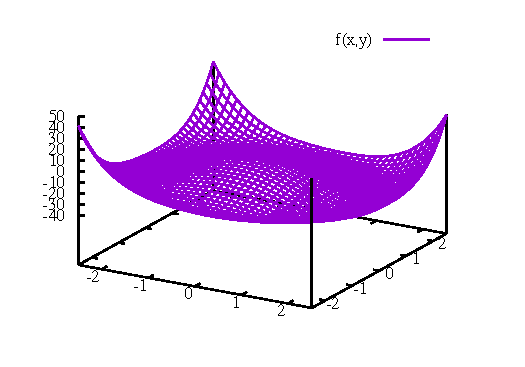
\includegraphics{image/func_2d.pdf}}
  \end{center}
\end{frame}

\begin{frame}[t,fragile]{様々な最適化手法の比較 (1/4)}
  \begin{center}
    \resizebox{.9\textwidth}{!}{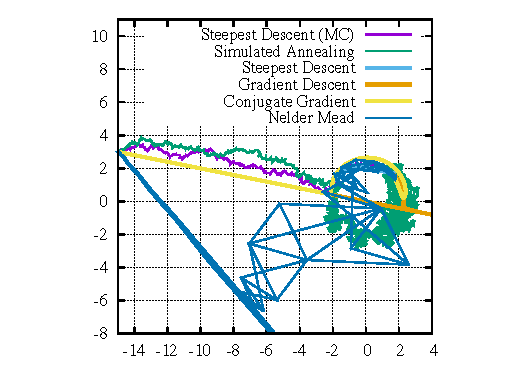
\includegraphics{image/optimization.pdf}}
  \end{center}
\end{frame}

\begin{frame}[t,fragile]{様々な最適化手法の比較 (2/4)}
  \begin{center}
    \resizebox{.9\textwidth}{!}{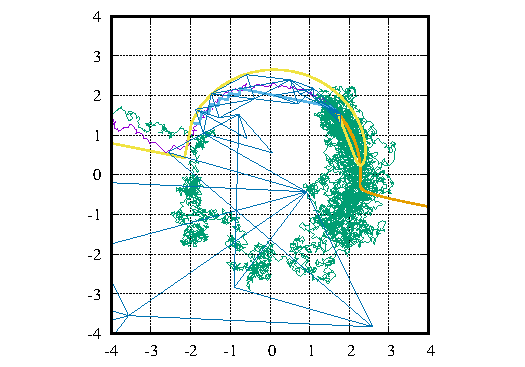
\includegraphics{image/optimization2.pdf}}
  \end{center}
\end{frame}

\begin{frame}[t,fragile]{様々な最適化手法の比較 (3/4)}
  \begin{center}
    \resizebox{.9\textwidth}{!}{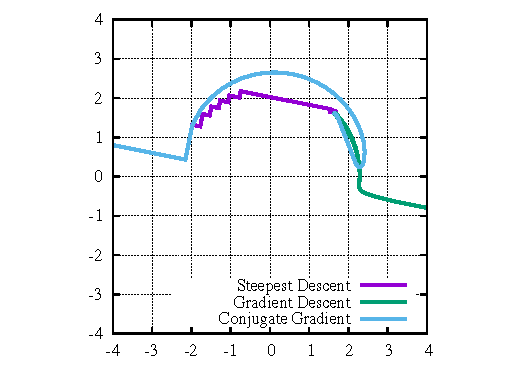
\includegraphics{image/optimization3.pdf}}
  \end{center}
\end{frame}

\begin{frame}[t,fragile]{様々な最適化手法の比較 (4/4)}
  \begin{center}
    \resizebox{.9\textwidth}{!}{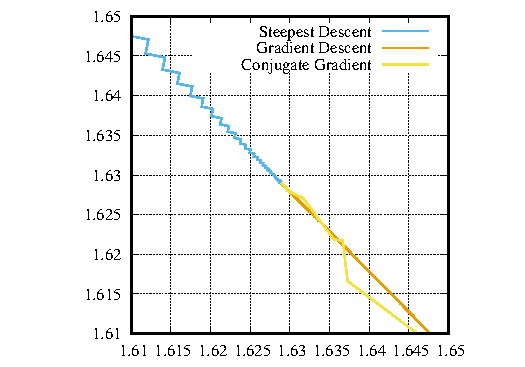
\includegraphics{image/optimization4.pdf}}
  \end{center}
\end{frame}

\begin{frame}[t,fragile]{真の解への近づき方}
  \begin{center}
    \resizebox{.9\textwidth}{!}{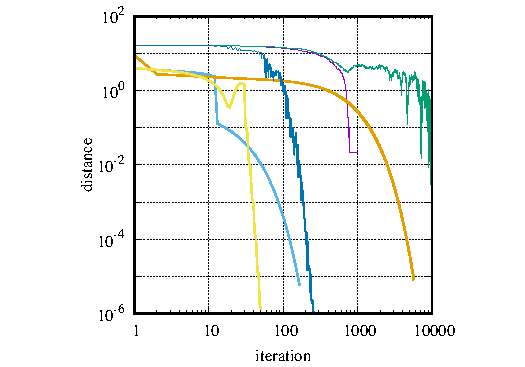
\includegraphics{image/convergence.pdf}}
  \end{center}
\end{frame}


\section{実習その3}

\begin{frame}[t,fragile]{EX3-1: サンプルプログラムの実行}
  \begin{itemize}
    %\setlength{\itemsep}{1em}
  \item[3-1-1] ガウスの消去法のサンプルプログラム(\href{https://github.com/todo-group/computer-experiments/blob/master/exercise/linear_system/gauss.c}{exercise/linear\_system/gauss.c})をコンパイル・実行せよ。実行時にコマンドライン引数に行列の内容が書かれたファイル名({\tt input1.dat})を指定する必要があることに注意
\begin{lstlisting}
$ cc gauss.c -o gauss
$ ./gauss input1.dat
\end{lstlisting}
  \item[3-1-2] LU分解のサンプルプログラム(\href{https://github.com/todo-group/computer-experiments/blob/master/exercise/linear_system/lu_decomp.c}{exercise/linear\_system/lu\_decomp.c})をコンパイル・実行せよ。コンパイル時にLAPACKをリンク({\tt -llapack})する必要があることに注意(ハンドブック3.1.6節)
\begin{lstlisting}
$ cc lu_decomp.c -o lu_decomp -llapack
$ ./lu_decomp input1.dat
\end{lstlisting}
  \end{itemize}
\end{frame}

\begin{frame}[t,fragile]{EX3-2: ピボット選択、境界条件}
  \begin{itemize}
    %\setlength{\itemsep}{1em}
  \item[3-2-1] {\tt gauss.c}では、ピボット選択を行っていないため、入力が{\tt input2.dat}の場合には正しい解が得られない。ピボット選択を行うよう{\tt gauss.c}を修正せよ
  \item[3-2-2] \href{https://github.com/todo-group/computer-experiments/blob/master/exercise/linear_system/laplace_lu.c}{exercise/linear\_system/laplace\_lu.c}では、ディリクレ型の境界条件[$u(0,y) = \sin(\pi y)$, $u(x,0)=u(x,1)=u(1,y)=0$]のもとでのラプラス方程式の解をLU分解により求めている。境界条件を変えてみて解がどのように変化するか、Gnuplotを用いてプロットして確認せよ(Gnuplotの{\tt splot}コマンドを使う)
  \end{itemize}
\end{frame}

\begin{frame}[t,fragile]{EX3-3: ヤコビ法、ガウス・ザイデル法、SOR法}
  \begin{itemize}
    %\setlength{\itemsep}{1em}
  \item[3-3-1] \href{https://github.com/todo-group/computer-experiments/exercise/blob/master/linear_system/laplace_jacobi.c}{exercise/linear\_system/laplace\_jacobi.c}は、作りかけのヤコビ法のプログラムである。収束判定のコードを追加し、プログラムを完成せよ。計算結果や計算速度を{\tt laplace\_lu.c}と比較せよ
  \item[3-3-2] ヤコビ法のプログラム({\tt lapalace\_jacobi.c})を元に、ガウス・ザイデル法、SOR法のプログラムを作成せよ。収束までの回数を比較せよ。
特にSOR法の場合、パラメータ$\omega$の選び方により、どのように収束回数が変化するか観察し、最適な$\omega$の値について考察せよ
  \end{itemize}
\end{frame}


\end{document}
